\chapter{Objectives Specification and Work Environment}

\section*{Introduction}
This chapter will first define the project's functional and non-functional requirements, then we will discuss the chosen structural decisions, explaining the reasoning behind their selection. Finally we will specify the hardware and software resources necessary for this project.

\section{Project Specification}
Requirements analysis is a fundamental phase in every project realization process. It is based on the study of the project's features as well as the constraints. In this section, we will cover both the functional and non-functional requirements.

\subsection{Functional Requirements}

The goal of the project is to generate a running CoreMark project on STM32 devices using CMSIS-Toolbox in an automated way. Within this context, this means guaranteeing the following concepts:

%\begin{itemize}
%    \item \textbf{Automation:} Ensuring that the user can generate a ready-to-build project without manually setting up peripheral configurations or memory layouts.
%    \item \textbf{Device Adaptability:} The project template must be dynamic in order to accomodate for the device specific characteristics of STM32 MCUs.
%    \item \textbf{CoreMark Integration:} CoreMark must be pre-configured and integrated within the project so that it can be executed immediately without further setup.
%    \item \textbf{Result Reporting:} The CoreMark results must be ouput in a standardized format, enabling consistent performance comparisons between devices.
%    \item \textbf{Multi-Toolchain Support:} The user should be able to build the project using any of the main embedded systems compilers without any extra configuration steps.
%\end{itemize}
%
%Table \ref{tab:functional_requirements} neatly summarizes the functional requirements for our project.

\begin{table}[htbp]
    \centering
    \caption{Functional Requirements for CMSIS-Toolbox based automated benchmarking}
    \label{tab:functional_requirements}
    \begin{tabularx}{\linewidth}{@{}>{\bfseries}l X X@{}}
        \toprule
        Requirements & Description \\
        \midrule
        Automation & The system must automatically generate a CoreMark benchmarking project for STM32 devices without requiring manual configuration. \\ \midrule
        Device Adaptability & The generated project must adapt to different STM32 families and configurations. \\ \midrule
        CoreMark Integration & The CoreMark benchmark must be integrated and ready to run immediately on the target hardware. \\ \midrule
        Result Reporting & The system must provide a standardized mechanism for reporting benchmark results. \\ \midrule
        Multi-Toolchain Support & The project must support multiple compilers such as GCC, ARM Compiler, and IAR. \\ \bottomrule
    \end{tabularx}
\end{table}
\subsection{Non-Functional Requirements}
Below are the non-functional requirements or the constraints that the functional expectations must abide by:
\begin{itemize}
    \item \textbf{Performance Requirements:}
    \begin{itemize}
        \item \textbf{Low Overhead} The project must not add significant, if any overhead besides the CoreMark runtime, this insures the integrity of the benchmarking results.
        \item \textbf{Compiler Optimizations} The project must provide the most optimal compiler configuration to ensure the maxmium performance results.
    \end{itemize}
   \item \textbf{Reliability Requirements:}
   \begin{itemize}
    \item \textbf{Correctness} The project must be functional and able to run without manual fixes.
    \item \textbf{Consistency} The project must produce consistent results amongst STM32 devices.
    \item \textbf{Error Handling} The project must fail gracefully and generate meaningful error messages.
   \end{itemize}
   \item \textbf{Usability Requirements:}
   \begin{itemize}
    \item \textbf{Ease of use} The generation process must be simple and intuitive, the project structure must be clear and consistent.
    \item \textbf{Standardized Output} The results must be presented in a clear format to facilitate further automation and data collection.
   \end{itemize}
\end{itemize}

\section{Structural Decisions}
Before delving further into the implementation details, it is crucial to understand the rationale behind the structural decisions chosen, for both the generation tool and the CoreMark project. This sections elucidates the reasons behind the choices and their relevence to the project's objectives.
\subsection{CoreMark Project}
The CoreMark project is the end result of the generation tool, it is meant to be runnable out of the box with the 3 main compilers (GCC, ARM, and IAR).

Ensuring the cross-toolchain support is done by providing the necessary compiler specific directives:
\begin{itemize}
	\item \textbf{Linker Scripts}
	Each compiler has their own unique format for linker scripts:
	\begin{itemize}
		\item \textbf{GCC:} GCC uses the .ld file extension and the LDScript syntax for the linking phase, it is structued in a declarative way to generate regions, sections and describe behavior within elements as well as exporting symbols.
		\item \textbf{IAR:} IAR uses the .icf file extension as well as proprietary syntax for the linking phase, it allows the user to simply declare regions and optionally sections and takes care of the rest.
		\item \textbf{ARM:} ARM compiler uses the .sct file extension, you only have to declare memory regions and the rest is handled either in C code or by the compiler directly.
	\end{itemize}
	\item \textbf{Startup Files} The startup file is written in assembly (this approach is changed in HAL2), and although most of the code is common between the 3 compilers, some specific instructions/symbols are different, as well as the libc initialization function is different as each compiler uses a different implementation.
	\item \textbf{Compiler Options} Each compiler has their own set of compiler flags to be used, providing each one with the appropriate configuration is crucial to ensure consistent running.
	\item \textbf{Generic Print Function Implementation} As mentioned prior, each compiler uses a different implementation of libc, meaning that the syscall behind the standard library's printf function are different, providing our own implementation and passing it to CoreMark for result reporting is the most efficient and platform-agnostic solution.
\end{itemize}
The table \ref{tab:cm_prj_struct} provides an overview of the architecture of the CoreMark project.
\begin{table}[H]
	\centering
   	\caption{CoreMark Project Structure}
   	\label{tab:cm_prj_struct}
   	\begin{tabularx}{\linewidth}{@{}>{\bfseries}l X X@{}}
    \toprule
    Element & Description \\
    \midrule
    User Code & This component provides the definition for the user application's entry point as well as the UART peripheral configuration. \\
    \midrule
    Driver & This component includes the necessary HAL drivers to enable the UART peripheral. \\
    \midrule
    Toolchain\_Specific & This component contains the toolchain specific source and header files to modify if the user wants to modify system configurations such as linker scripts and startup files. \\
    \midrule
    CoreMark & This component contains the source code of the CoreMark benchmark to be invoked within the usercode's entry point. \\
    \midrule
    coremark.csolution.yml & This is the workspace file for CMSIS-Toolbox to have knowledge of the project, it defines the DFP, ARM's CORE component, alongside the target device, build types and compiler selection. \\
    \midrule
    coremark.cproject.yml & This is the project description file, it contains the source files to be compiled, user defines for UART functionality and the include paths. \\
    \midrule
    cdefault.yml & This is the file that contains all the compiler options, in our context, the configuration is meant to provide the most performance-oriented setup. \\
    \bottomrule
   \end{tabularx}
\end{table}


\subsection{Project Generation Tool}
The architecture of the CoreMark project is quite complex and contains multiple pieces that must be either generated dynamically or fetched from different resources.
\begin{figure}[H]
    \centering
    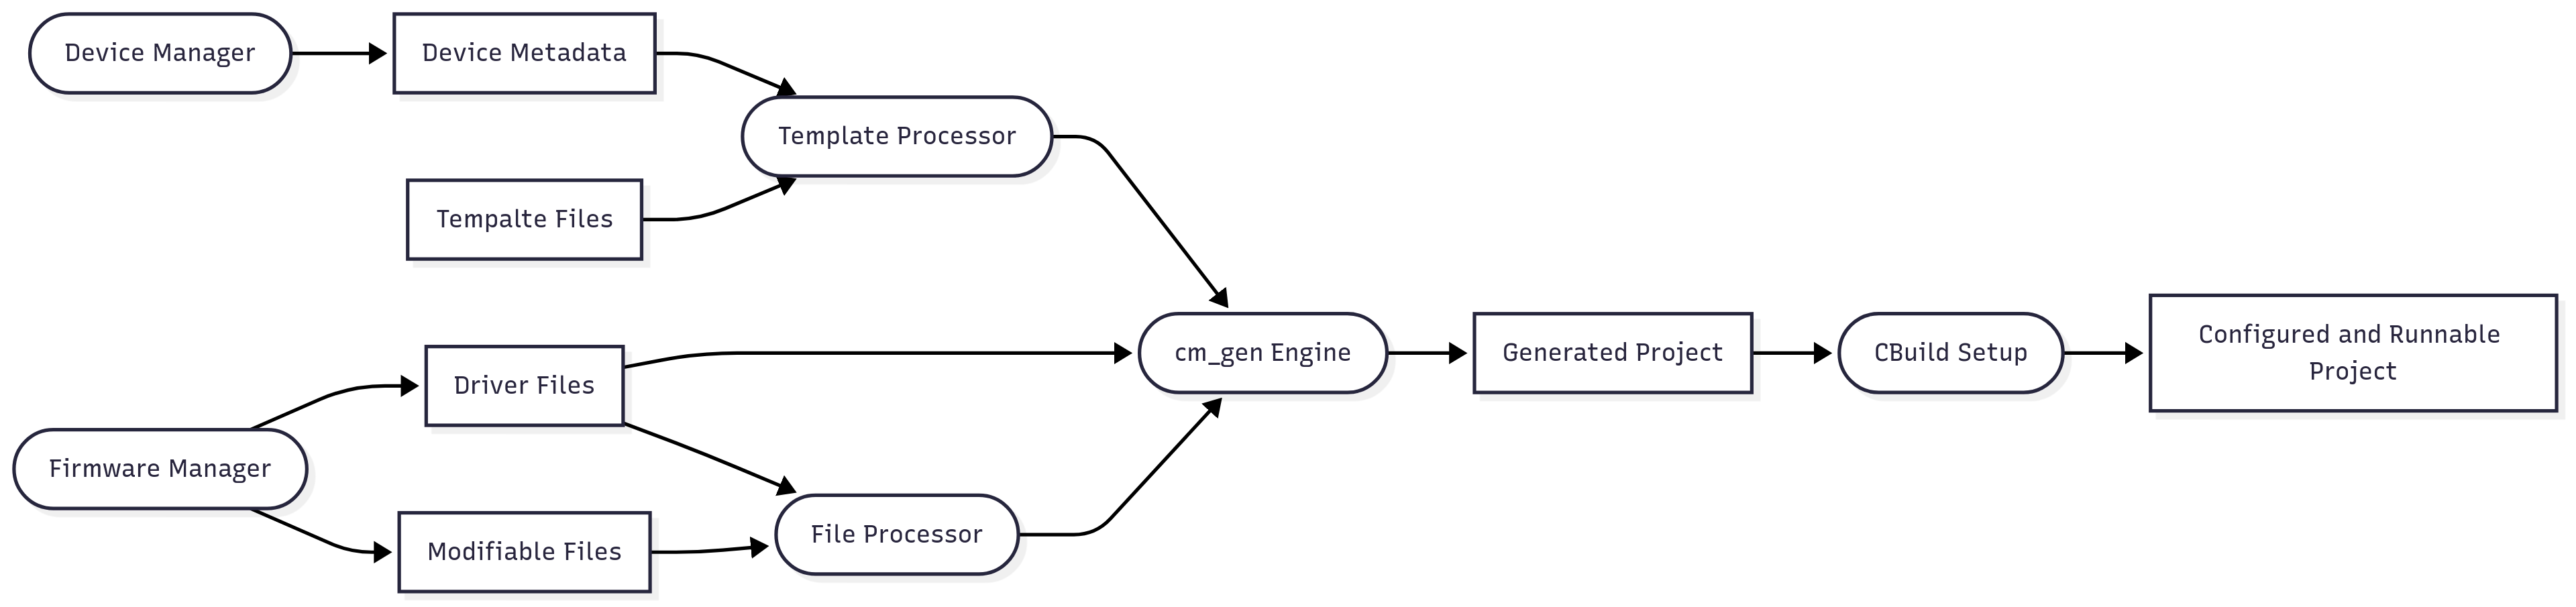
\includegraphics[width=15cm]{ST_Summer_Internship/GenerationToolComponents.png}
    \caption{Project Generation Tool Architecture}
    \label{fig:gen_tool_arch}
\end{figure}
The figure \ref{fig:gen_tool_arch} shows the multiple modules within the project generation tool.
\begin{table}[htbp]
   \centering
   \caption{Project Generation Tool Structure}
   \begin{tabularx}{\linewidth}{@{}>{\bfseries}l X X@{}}
    \toprule
    Module & Description \\
    \midrule
       Device Manager & Extracts the device metadata \\
    \midrule
       Firmware Manager & Manages the device's firmware pack and extracting the necessary files \\
    \midrule
       Template Processor & Generates files from the template files and the gathered data \\
    \midrule
       File Processor & Modifies firmware files that cannot be templated to accomodate for our project's context \\
    \midrule
       cm\_gen Engine & Orchestrates and runs the different modules \\
    \bottomrule
   \end{tabularx}
\end{table}

\section{Use-Case Diagram}

\begin{figure}[H]
	\centering
	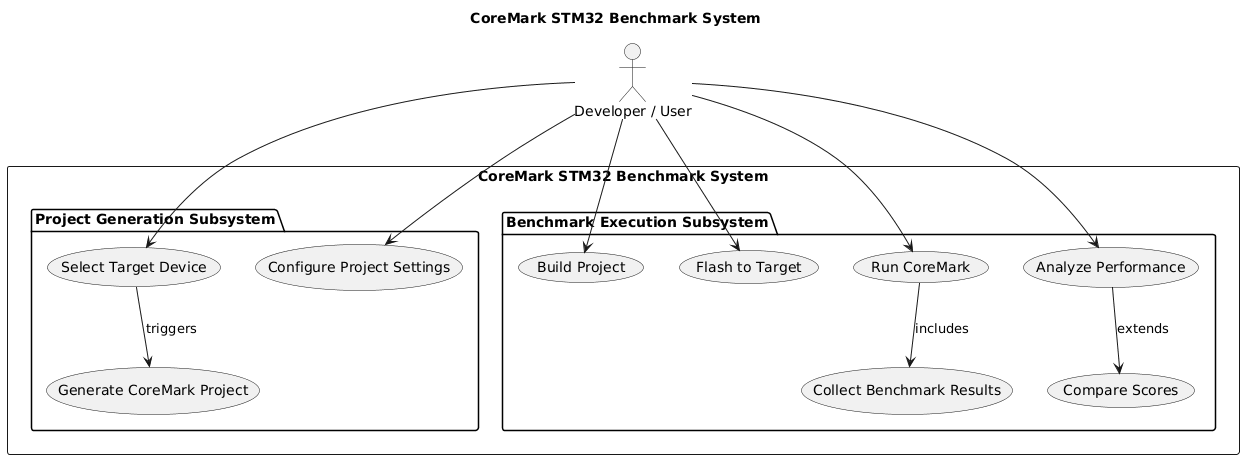
\includegraphics[width=15cm]{img/ST_Summer_Internship/use_case2.png}
	\caption{Automated CoreMark Benchmarking Use-Case Diagram}
	\label{fig:use_case_diagram}
\end{figure}

The Use-Case diagram in Figure \ref{fig:use_case_diagram} illustrates the interactions between a user, the project generation tool and the project's execution space.
Refer to Table \ref{tab:use_cases} for an in-depth explanation:

\begin{xltabular}{\linewidth}{@{}>{\bfseries}l X@{}}
	\caption{Automated CoreMark Benchmarking\label{tab:use_cases}} \\
	\toprule
	\textbf{Use Case} & \textbf{Relevance} \\
	\midrule
	\endfirsthead % Header for first page
	
	\multicolumn{2}{c}{{\tablename\ \thetable{} -- Continued from previous page}} \\
	\toprule
	\textbf{Use Case} & \textbf{Relevance} \\
	\midrule
	\endhead % Header for subsequent pages
	
	\midrule
	\multicolumn{2}{r}{{Continued on next page}} \\
	\endfoot % Footer for all pages except last
	
	\bottomrule
	\endlastfoot % Footer for the last page
	
	\multicolumn{2}{ c }{\textbf{Project Generation Subsystem}} \\
	\midrule
	Select Target Device &
	The developer selects the STM32 device or family for which the CoreMark project should be generated. 
	This ensures that the automation tool generates the correct configuration files and CMSIS device support. \\
	\midrule
	Configure Project Settings &
	The developer configures CoreMark-specific parameters such as iteration counts, seed values, and compiler optimization flags 
	before building and running the benchmark. \\
	\midrule
	Generate CoreMark Project &
	The automation tool generates a complete project structure, including the \texttt{csolution} files and necessary source code, 
	ready to be built and deployed for the selected STM32 target. \\
	\midrule
	\multicolumn{2}{ c }{\textbf{CoreMark Project Subsystem}} \\
	\midrule
	Build Project &
	The CoreMark project is compiled using the CMSIS build system and toolchain to produce a firmware image for the target hardware. \\
	\midrule
	Flash Target &
	The compiled binary is flashed to the STM32 device to prepare it for execution.\\
	\midrule
	Run CoreMark &
	The benchmark executes on the STM32 target, performing operations such as list processing, matrix manipulation, and state machine handling 
	to measure CPU performance. \\
	\midrule
	Collect CoreMark Results &
	During execution, CoreMark outputs the cycle count, execution time, and final score. \\
	\midrule
	Analyze Performance &
	The developer interprets the CoreMark/MHz score and other performance metrics to determine how well the device performs within the specified context. \\
	\midrule
	Compare Scores &
	Performance results are compared across different devices, toolchains, or configurations to guide hardware selection or optimization decisions.
\end{xltabular}

\section*{Work Environment}
In this section, we outline the hardware and software resources utilized during the internship project that were essential for the development testing, and validation.

\section{Hardware Resources}
\begin{figure}[H]
	\centering
	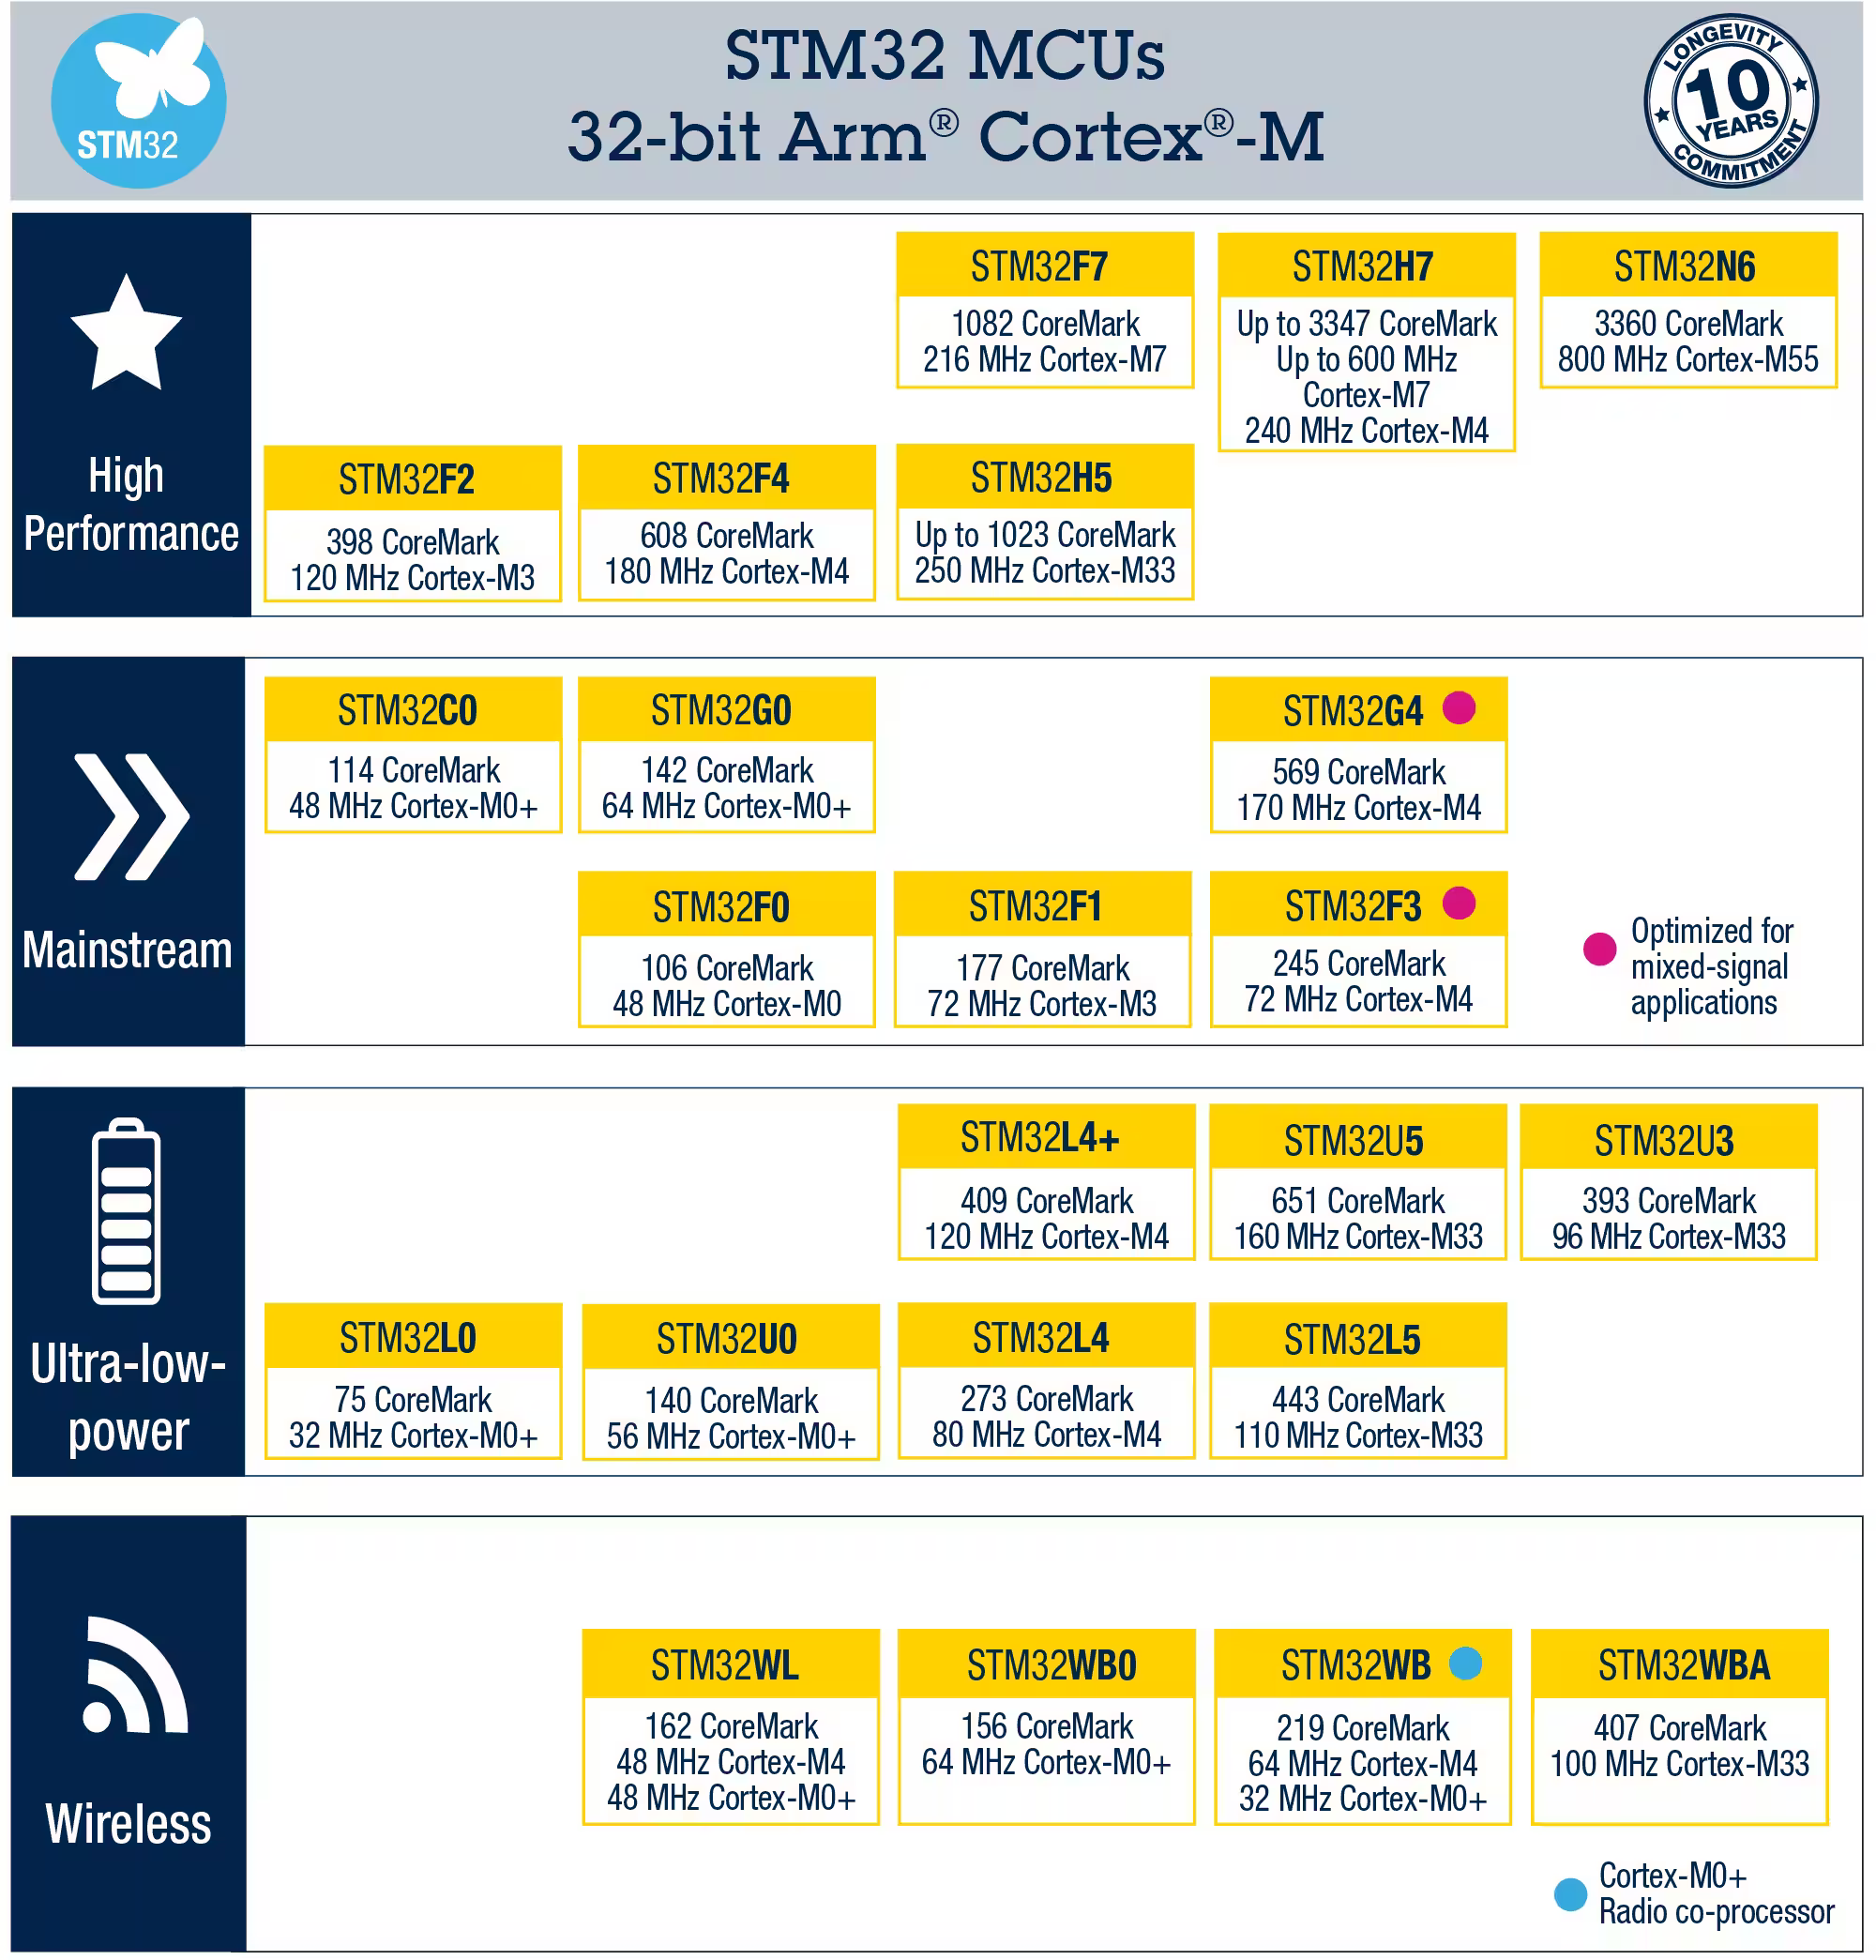
\includegraphics[width=15cm]{img/ST_Summer_Internship/arm_cortex_mcu_portfolio.png}
	\caption{STM32 Microcontroller Portfolio}
	\label{fig:stm32_portfolio}
\end{figure}
The project is meant to work on all STM32 MCUs, therefore as a base unit, the validation was done on a single board from all STM32 MCU families.
Table \ref{tab:stm32_mcu_families} describes all the available families:
\begin{xltabular}{\linewidth}{@{}>{\bfseries}l X@{} X@{} X@{} X@{} X@{}}
	\caption{STM32 Microcontroller Families\label{tab:stm32_mcu_families}} \\
	\toprule
	\textbf{Family} & \textbf{Core} & \textbf{Maximum Frequency(MHz)} & \textbf{Read-Only Memory} & \textbf{Random Access Memory} & \textbf{Additional Features} \\
	\midrule
	\endfirsthead % Header for first page
	
	\multicolumn{6}{c}{{\tablename\ \thetable{} -- Continued from previous page}} \\
	\toprule
	\textbf{Family} & \textbf{Core} & \textbf{Maximum Frequency} & \textbf{Read-Only Memory} & \textbf{Random Access Memory} & \textbf{Additional Features} \\
	\midrule
	\endhead % Header for subsequent pages
	
	\multicolumn{6}{r}{{Continued on next page}} \\
	\endfoot % Footer for all pages except last
	
	\bottomrule
	\endlastfoot % Footer for the last page
	
	STM32C0 &
	Arm Cortex-M0+ &
	48MHZ & 16-256KB & 6-36KB & - \\
	\midrule
	STM32F0 &
	Arm Cortex-M0 &
	48MHz & 16-256KB & 4-32KB & - \\
	\midrule
	STM32F1 &
	Arm Cortex-M3 &
	72MHz & 16KB-1MB & 4-96KB & - \\
	\midrule
	STM32F2 &
	Arm Cortex-M3 &
	120MHz & 128KB-1MB & 64KB-128KB & ART Accelerator \\
	\midrule
	STM32F3 &
	Arm Cortex-M4 &
	72MHz & 32-512KB & 16-80KB & CCM-SRAM and FPU/DSP instructions \\
	\midrule
	STM32F4 &
	Arm Cortex-M4 &
	180MHz & 64KB-2MB & 32-384KB & Chrom-ART Accelerator\\
	\midrule
	STM32F7 &
	Arm Cortex-M7 &
	216MHz & 64K-2MB & 256-512KB & L1 Data and Instruction Caches, TCM, Read-While-write Flash capabilities \\
	\midrule
	STM32G0 &
	Arm Cortex-M0+ &
	64MHz & 16-512KB & 8-144KB & \\
	\midrule
	STM32G4 &
	Arm Cortex-M4 &
	170MHz & 32-512KB & 32-128KB & CCM-SRAM and FPU/DSP instructions \\
	\midrule
	STM32H5 &
	Arm Cortex-M33 &
	250MHz & 128KB-2MB & 32-640KB & Integrated Instruction and Data Cache peripherals \\
	\midrule
	STM32H7 &
	Arm Cortex-M7 &
	600MHz & 64KB-2MB & 536KB-1.4MB & L1 Data and Instruction Cache, TCM, Chrome-ART and NeoChrom Accelerators.  \\
	\midrule
	STM32L0 &
	Arm Cortex-M0+ &
	32MHz & 8-192KB & 2-20KB & Up to 6KB of EEPROM \\
	\midrule
	STM32L1 &
	Arm Cortex-M3 &
	32MHz & 32-512KB & 4-80KB & Up to 16KB of EEPROM \\
	\midrule
	STM32L4 &
	Arm Cortex-M4 &
	80MHz & 64KB-1MB & 40-320KB & Chrom-ART Accelerator \\
	\midrule
	STM32L4+ &
	Arm Cortex-M4 &
	120MHz & 512KB-2MB & 320-640KB & Chrom-ART Accelerator \\
	\midrule
	STM32L5 &
	Arm Cortex-M33 &
	110MHz & 256-512MB & 256KB & ART Accelerator \\
	\midrule
	STM32N6 &
	Arm Cortex-M55 &
	800MHz & 0 & 4.2MB & Neural-ART Accelerator(Up to 1GHz Clock Speed) \\
	\midrule
	STM32U0 &
	Arm Cortex-M0+ &
	56MHz & 16-256KB & 12-40KB & - \\
	\midrule
	STM32U3 &
	Arm Cortex-M33 &
	96MHz & 512KB-1MB & 256KB & Integrated Instruction and Data Cache peripherals \\
	\midrule
	STM32U5 &
	Arm Cortex-M33 &
	160MHz & 128-4MB & 274KB-3MB & Integrated Instruction and Data Cache peripherals \\
	\midrule
	STM32WB &
	Arm Cortex-M4 &
	64MHz & 256KB-1MB & 48-256KB & - \\
	\midrule
	STM32WB0 &
	Arm Cortex-M0+ &
	64MHz & 192-512KB & 24-64KB & - \\
	\midrule
	STM32WBA &
	Arm Cortex-M33 &
	100MHz & 512KB-2MB & 64-512KB & Integrated Instruction and Data Cache peripherals \\
	\midrule
	STM32WL &
	Arm Cortex-M4 &
	64MHz & 64-256KB & 8-64KB & - \\
	
\end{xltabular}

\section{Software Resources}
The following software tools were used for the  development, debugging and testing of the project:
\subsection{Programming Languages}
\begin{itemize}
	\item \textbf{C:}
	 C is a general-purpose programming language. By design, it gives the programmer relatively direct access to the features of the typical CPU architecture, customized for the target instruction set. It has been and continues to be used to implement operating systems (especially kernels), device drivers, protocol stacks, and embedded applications. C is used on computers that range from the largest supercomputers to the smallest microcontrollers. 
	\item \textbf{Go:}
	 Go (or Golang) is a high-level general purpose programming language that is statically typed and compiled. It is known for the simplicity of its syntax and the efficiency of development that it enables by the inclusion of a large standard library supplying many needs for common projects.
	\item \textbf{Python:}
	 Python is a high-level, general-purpose programming language. Its design philosophy emphasizes code readability with the use of significant indentation.
	 Python is dynamically type-checked and garbage-collected. It supports multiple programming paradigms, including structured (particularly procedural), object-oriented and functional programming. 
\end{itemize}
\subsection{Integrated Development Environments and Text Editors}
\subsubsection{Visual Studio Code}
Visual Studio Code (VS Code) is an extensible code editor developed by Microsoft for Windows, Linux, macOS and web browsers. Features include support for debugging, syntax highlighting, intelligent code completion, snippets, code refactoring, and embedded version control with Git. Users can install extensions that add functionality.
Table \ref{tab:vscode_extensions} goes over the most impactful extensions during the development of the project.
\begin{xltabular}{\linewidth}{@{}>{\bfseries}l X@{}}
	\caption{Relevant VSCode Extensions\label{tab:vscode_extensions}} \\
	\toprule
	\textbf{Extension} & \textbf{Description} \\
	\midrule
	\endfirsthead % Header for first page
	
	\multicolumn{2}{c}{{\tablename\ \thetable{} -- Continued from previous page}} \\
	\toprule
	\textbf{Extension} & \textbf{Description} \\
	\midrule
	\endhead % Header for subsequent pages
	
	\multicolumn{2}{r}{{Continued on next page}} \\
	\endfoot % Footer for all pages except last
	\bottomrule
	\endlastfoot % Footer for the last page
	
	Arm CMSIS Solution & The Arm CMSIS Solution extension is a graphical user interface for csolution projects that use the CMSIS-Toolbox. The extension supports microcontroller devices that incorporate Arm Cortex®-M processors and works with various C/C++ compilers and debuggers.\\
	\midrule
	Arm CMSIS Debugger & The Arm CMSIS Debugger extension pack is a comprehensive debug platform for Arm Cortex-M processor-based devices that uses the GDB/MI protocol. It supports single and multi-core processor systems, it includes pyOCD for target connection and image download, as well as GDB for core debugging features.\\
	\midrule
	Serial Monitor & The Serial Monitor extension provides a serial monitor to view output from as well as send messages to serial ports. This is often useful when testing or debugging programs on embedded devices. \\
	\midrule
	ELFInsight & ElfInsight is an extension to analyze ARM Cortex-M ELF files, it offers a streamlined interface to view symbol tables, inspect memory usage and visualize function call graph.\\
\end{xltabular}
\subsection{Compiler Toolchains}
\subsubsection{GCC}
The GCC compiler is an open-source C/C++ compiler, and is part of the GNU utilities, ARM provides their own implementation, prefixed with "arm-none-eabi" and can target most ARM architectures such as ARMv7 and ARMv8.
\subsubsection{ARM Compiler v6}
As well as providing a cross-compiling gcc toolchain, ARM has their own compiler based on CLANG and LLVM technologies called ARM compiler.
\subsubsection{IAR Toolchain}
IAR Systems is a Swedish computer software company that offers development tools for embedded systems. They are known for having a comprehensive development suite and an optimized compiler based on GCC.
\subsection{Development Tools}
\subsubsection{CMake}
CMake is a free, open-source, cross-platform, software development tool for building applications via compiler-independent instructions. It also can automate testing, packaging and installation. It runs on a variety of platforms and supports many programming languages.
As a meta-build tool, CMake configures native build tools which in turn build the codebase. CMake generates configuration files for other build tools based on CMake-specific configuration files. The other tools are responsible for more directly building; using the generated files. A single set of CMake-specific configuration files can be used to build a codebase using the native build tools of multiple platforms.
\subsubsection{Ninja}
Ninja is a small build system with a focus on speed. It differs from other build systems in two major respects: it is designed to have its input files generated by a higher-level build system, and it is designed to run builds as fast as possible.
\subsubsection{CMSIS-Toolbox}
The CMSIS-Toolbox provides command-line tools for project creation and build of embedded applications utilizing CMSIS-Packs. It supports multiple compilation tools. It also helps with software pack creation, maintenance, and distribution utilizing the CMSIS-Pack format.
\subsubsection*{Overall Workflow}
The CMSIS-Toolbox includes the following tools for the creation of embedded applications:
\begin{itemize}
	\item \textbf{ Pack Manager (cpackget):} install and manage software packs in the host development environment.
	\item \textbf{Project Manager (csolution):} create build information for embedded applications that consist of one or more related projects. It performs the following operations:
	\begin{itemize}
		\item \textbf{In the Project Area:} Generate build information files *.cbuild-idx.yml and *.cbuild.yml with all relevant project information for the build process.
		\item \textbf{In the RTE Directory:}
		\begin{itemize}
			\item Generate for each context the RTE\_components.h file and pre-include files from the software pack (*.pdsc) metadata.
			\item Copy the configuration files from selected software componentsand provide PLM information.
		\end{itemize}
	\end{itemize}
	\begin{figure}[H]
		\centering
		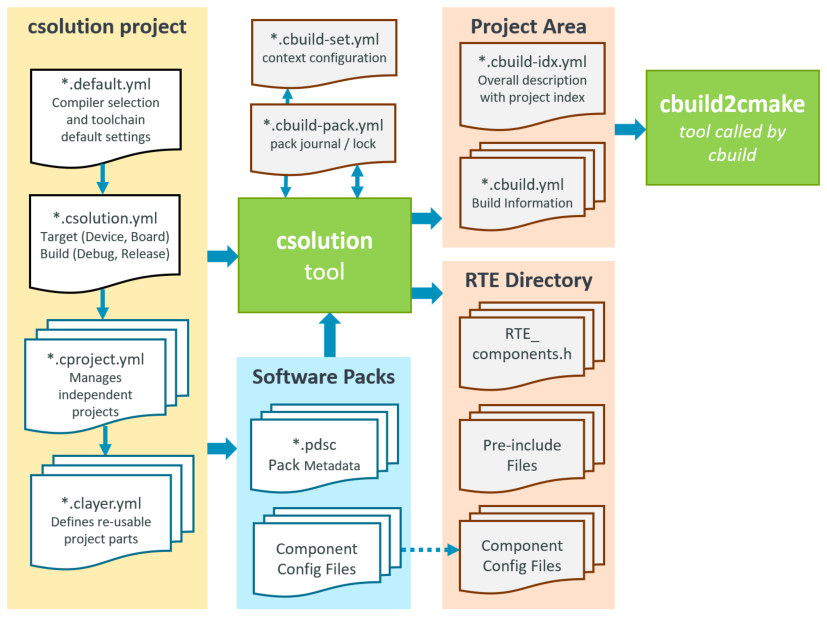
\includegraphics[width=15cm]{img/ST_Summer_Internship/csolution-operation.png}
		\caption{Csolution Operation}
		\label{fig:csolution_op}
	\end{figure}    
	\item \textbf{Build Invocation (cbuild):} orchestrate the build steps utilizing CMSIS tools and a CMake compilation process. It has two overall modes :
	\begin{itemize}
		\item \textbf{build mode:} generates the application and is the default command.
		\begin{itemize}
			\item When option --packs is used, it downloads missing software packs using cpackget.
			\item It calls csolution to process the the <name>.csolution.yml project. The output are build information files with all relevant project information for the build process.
		\end{itemize}
		\item  \textbf{setup mode:} generates the setup information for an IDE to populate dialogues, IntelliSense, and project outline views.
		\begin{itemize}
			\item Check YML file syntax against schema for all files specified by *.csolution.yml.
			\item Check the correctness of all files specified by *.csolution.yml.
		\end{itemize}
	\end{itemize}
	\begin{figure}[H]
		\centering
		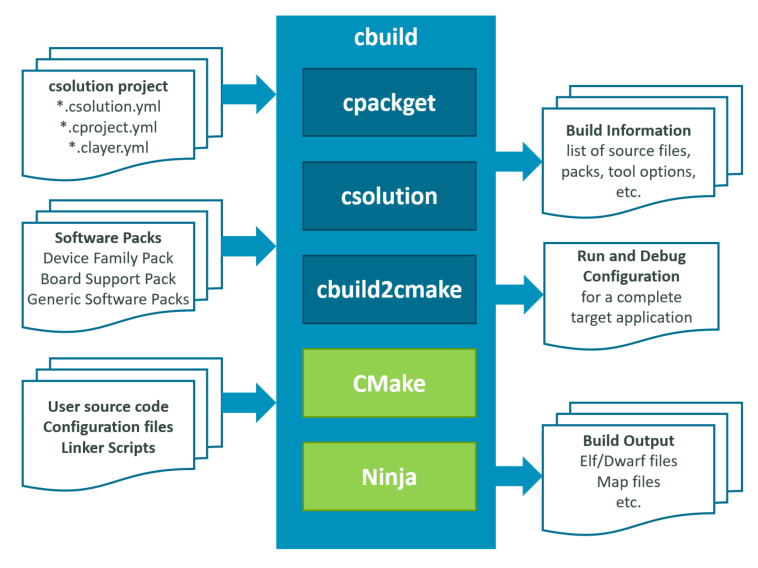
\includegraphics[width=15cm]{img/ST_Summer_Internship/cbuild-workflow.png}
		\caption{Cbuild Workflow}
		\label{fig:cbuild_wf}
	\end{figure}
\end{itemize}
\subsubsection{PyOCD}
pyOCD is an open source Python based tool and package for programming and debugging Arm Cortex-M microcontrollers with a wide range of debug probes. It is fully cross-platform, with support for Linux, macOS, Windows, and FreeBSD.
Beyond its standalone capabilities, pyOCD has been integrated into the CMSIS-Toolbox ecosystem as a backend for device flashing and debugging. As a result, it simplifies the automation of programming and debugging tasks across different hardware targets and development environments.
\begin{figure}[H]
	\centering
	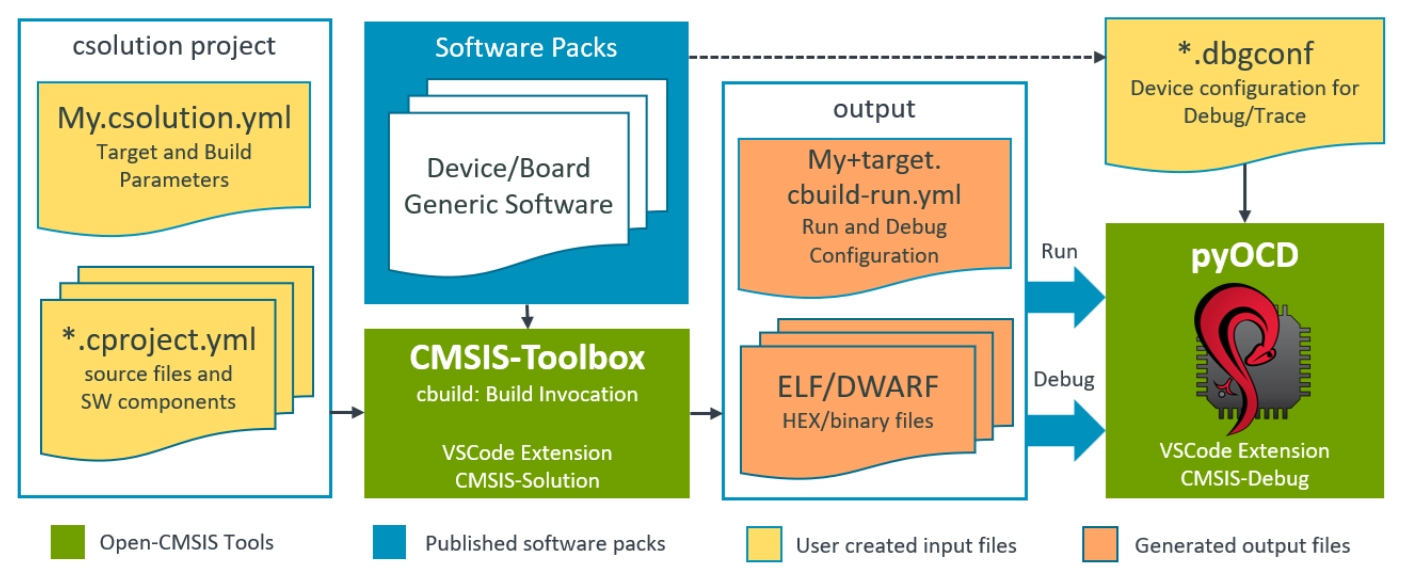
\includegraphics[width=15cm]{img/ST_Summer_Internship/cbuild-run.png}
	\caption{PyOCD CMSIS-Toolbox-Integrated Running and Debugging Workflow}
	\label{fig:debug_wf}
\end{figure}
The CMSIS-Toolbox uses the information from the DFP and BSP to simplify the debugger configuration. It generates the file *.cbuild-run.yml that contains for one target of a csolution project all information for run and debug.
The software packs contain information that is the basis for debug and run settings:
\begin{itemize}
	\item Flash algorithms of device memory (in DFP) and board memory (in BSP).
	\item On-board debug adapter (a default programming/debug channel) including features.
	\item Available memory of device and board.
	\item Device parameters such as processor core(s) and clock speed.
	\item Debug Access Sequences and System Description Files.
	\item Debug Configuration files (*.dbgconf) that configure device properties such as trace pins.
	\item CMSIS-SVD SVD files for viewing device peripherals.
	\item CMSIS-View SCVD files for analysis of software components (RTOS, Middleware).
\end{itemize}
\subsubsection{STM32CubeProgrammer}
STM32CubeProgrammer is a proprietary, all-in-one programming tool provided by STMicroelectronics that facilitates the flashing and configuration of STM32 microcontrollers. Supporting a wide array of connectivity options, it offers a unified interface for erasing, programming, and verifying device memory across the entire STM32 portfolio. The tool provides advanced features like secure programming, option byte management, and lifecycle management for TrustZone-enabled devices. Its support for scripting and CLI operation further enables automation in production and development environments.
\subsubsection{STM32CubeMX}
STM32CubeMX is a graphical software configuration tool that simplifies the development of STM32-based applications. It allows developers to:
\begin{itemize}
	\item Configure microcontroller peripherals and middleware components through an intuitive graphical interface.
	\item Generate initialization code for STM32 microcontrollers, reducing development time.
	\item Integrate with various IDEs, including IAR Embedded Workbench, for a streamlined development workflow.
\end{itemize}
\section*{Conclusion}
The work environment for this internship includes both hardware and software resources that are essential for the successful implementation of the project.
